% ===========================================================================
% Figura 1.1: Sincronización de reloj unidireccional y bidireccional
% Basada en la Figura 1.1 del documento base TD_Malcolm_Eupierre.pdf
% ===========================================================================
\documentclass[tikz,border=10pt]{standalone}
\usepackage[utf8]{inputenc}
\usepackage[T1]{fontenc}
\usepackage{lmodern}
\usepackage{amsmath}
\usetikzlibrary{shapes.geometric, arrows.meta, positioning, calc}

\begin{document}
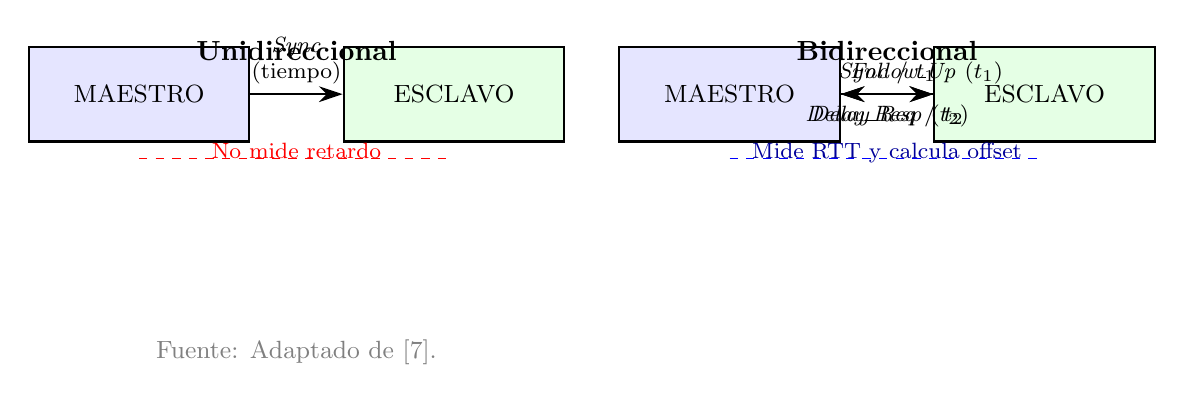
\begin{tikzpicture}[
    node distance=1.5cm,
    block/.style={rectangle, draw, thick, minimum width=2.8cm, minimum height=1.2cm, align=center, font=\small},
    arrow/.style={-{Stealth[length=3mm,width=2mm]}, thick},
    label/.style={font=\footnotesize, align=center}
  ]

  % ---- LEFT: Unidireccional ----
  \begin{scope}[local bounding box=uni]
    \node[block, fill=blue!10] (m1) at (0,0) {MAESTRO};
    \node[block, fill=green!10] (s1) at (4,0) {ESCLAVO};

    \draw[arrow] (m1.east) -- node[above, label] {\emph{Sync} \\ (tiempo)} (s1.west);
    \node[above=0.3cm of $(m1)!0.5!(s1)$] {\textbf{Unidireccional}};

    % Nota
    \node[below=0.5cm of $(m1)!0.5!(s1)$, label, text=red] {No mide retardo};
    \draw[red, dashed] ($(m1.south)+(0,-0.2)$) -- ($(s1.south)+(0,-0.2)$);
  \end{scope}

  % ---- RIGHT: Bidireccional ----
  \begin{scope}[xshift=7.5cm, local bounding box=bi]
    \node[block, fill=blue!10] (m2) at (0,0) {MAESTRO};
    \node[block, fill=green!10] (s2) at (4,0) {ESCLAVO};

    \draw[arrow] (m2.east) -- node[above, label] {\emph{Sync} / $t_1$} (s2.west);
    \draw[arrow, dashed] (s2.west) -- node[below, label] {\emph{Delay\_Req} / $t_2$} (m2.east);
    \draw[arrow] (m2.east) -- node[above, label, xshift=0.5cm] {\emph{Follow\_Up} ($t_1$)} (s2.west);
    \draw[arrow, dashed] (s2.west) -- node[below, label] {\emph{Delay\_Resp} ($t_2$)} (m2.east);

    \node[above=0.3cm of $(m2)!0.5!(s2)$] {\textbf{Bidireccional}};
    \node[below=0.5cm of $(m2)!0.5!(s2)$, label, text=blue!60!black] {Mide RTT y calcula offset};
    \draw[blue, dashed] ($(m2.south)+(0,-0.2)$) -- ($(s2.south)+(0,-0.2)$);
  \end{scope}

  % Etiquetas generales
  \node[font=\small, text=gray, below] at (2,-3) {Fuente: Adaptado de [7].};
\end{tikzpicture}
\end{document}
